\chapter{Detección de biomarcadores en cáncer de hígado y colon-recto}

\section{Objetivos}

El objetivo general consiste en intentar predecir en base a pocos genes si una enfermedad padece o no cáncer de hígado, o cáncer de colon-recto. Para ello se usarán distintas técnicas de selección de características: mRMR, RF y DA, así como varios algoritmos de clasificación: SVM, RF y kNN.

\section{Metodología}

\subsection{Fuente de datos}

La fuente de los datos es GDC (Genomic Data Commons) Portal, una plataforma web sobre cáncer del Instituto Nacional del Cáncer de Estados Unidos (\textit{National Cancer Institute}) \cite{GDCPortal, NationalCancerInstitute}. GDC Portal fue desarrollado por el Instituto Nacional del Cáncer de Estados Unidos, la Universidad de Chicago, el Instituto de Ontario para la Investigación del Cáncer y la empresa \textit{Leidos Biomedical Research}, y su principal fortaleza reside en la integración y armonización de diversas fuentes heterogéneas, creando así un sistema de información amplio y robusto \cite{Grossman2016}. \\

\newpage
\textbf{\textcolor{red}{Figura XX}}. Diagrama de funcionalidad y utilidad de GDC. Extraído de Grossman et al. \cite{Grossman2016}.
\begin{center}
	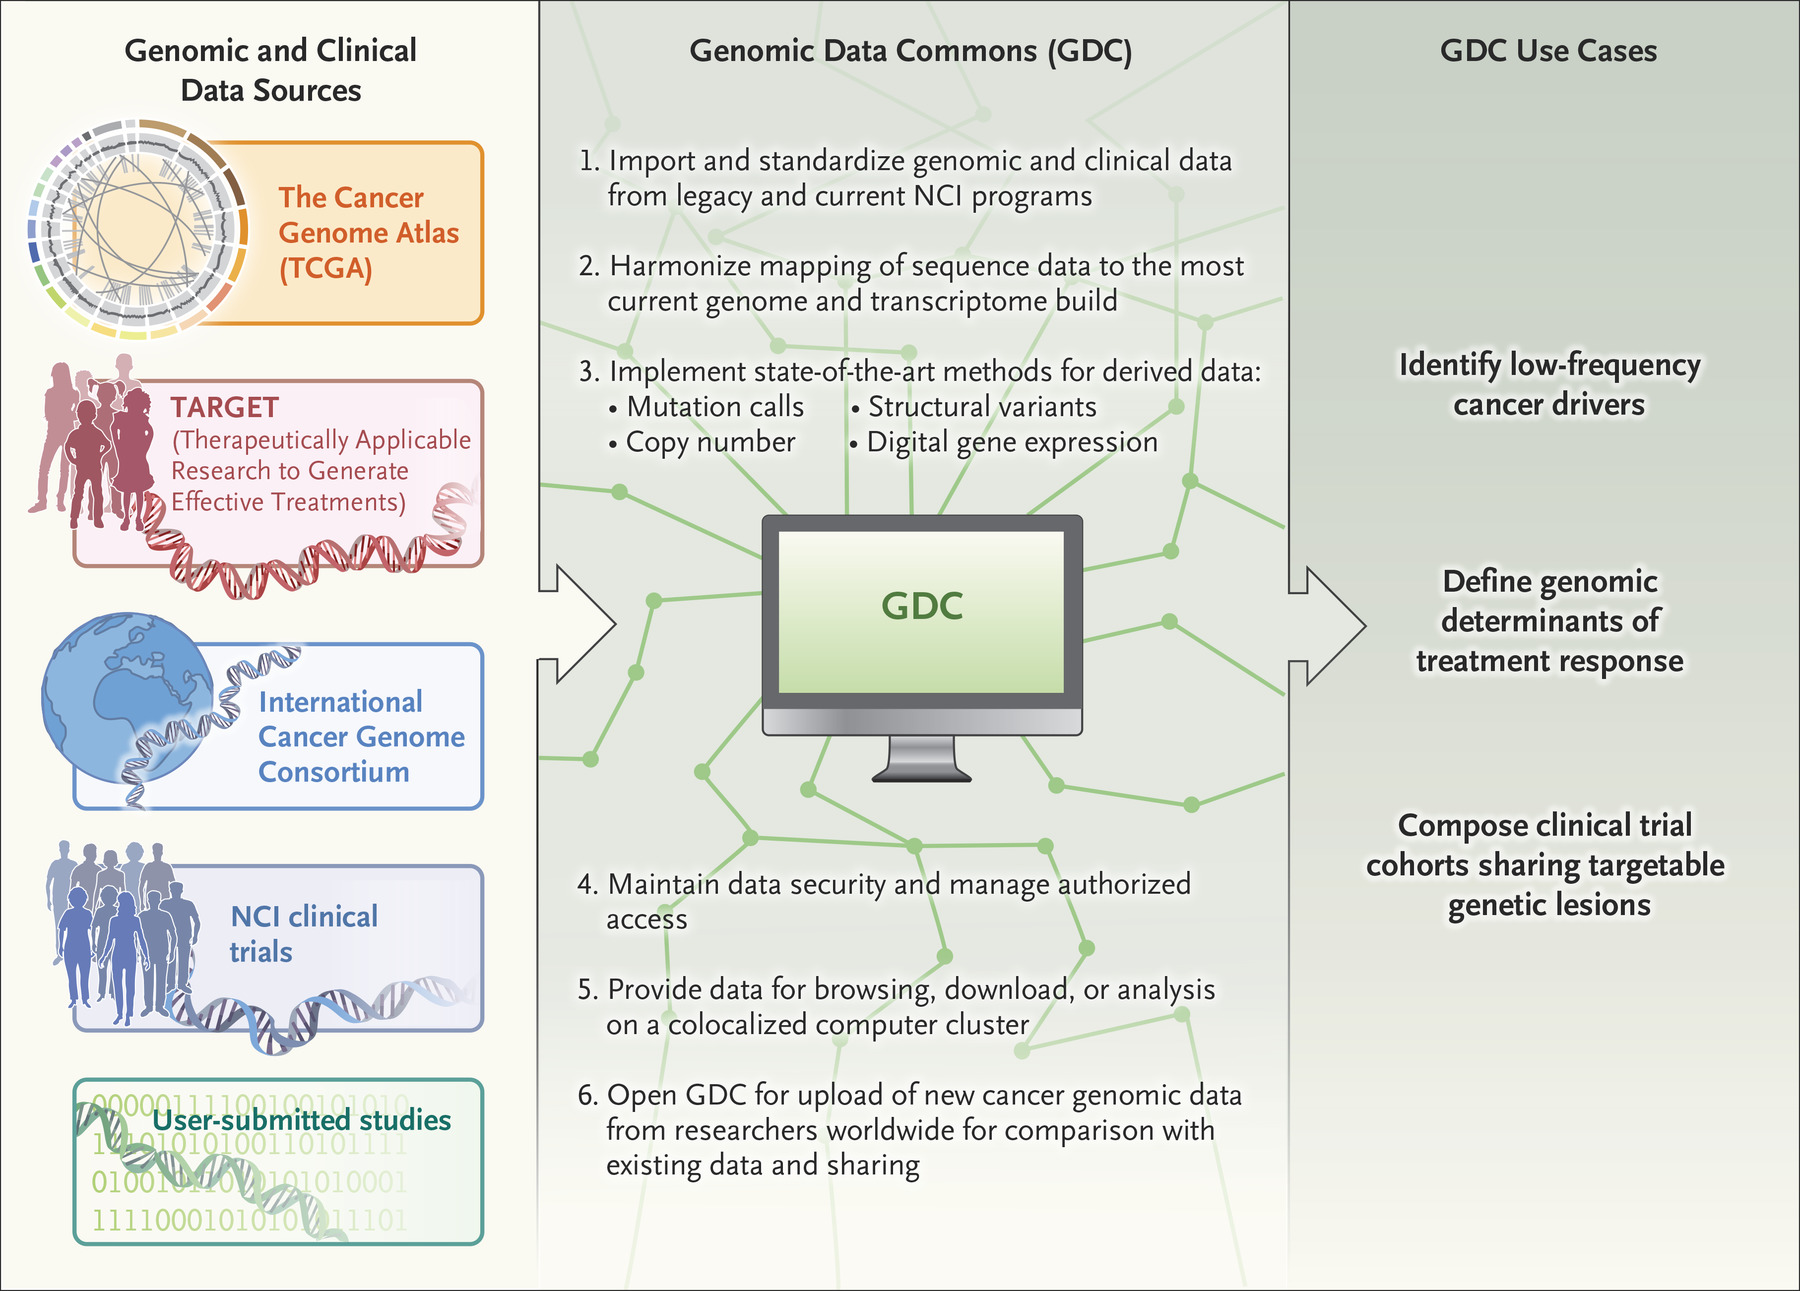
\includegraphics[width=1\textwidth]{figuras/funcionamiento_gdc.jpeg} \\
\end{center}

GDC Portal, a día 22 de Junio, contenía información sobre unos 84.000 casos, 23.000 genes y más de 3 millones de mutaciones de genes \cite{GDCPortal}. Algunos de estos datos son abiertos, mientras que para otros es necesario solicitar acceso. Los datos de los que dispone son muy variados, y se pueden distinguir en tres grandes categorías:

\begin{itemize}
	\item Información clínica, como la edad del sujeto, su sexo o el estadio del cáncer del que ha sido diagnosticado.
	\item Información genética y transcriptómica proveniente de diversos proyectos de investigación.
	\item Imágenes de tejidos tumorales y sanos.
\end{itemize} 

Para el presente trabajo se han descargado de GDC Portal todos los datos que cumplen las siguientes condiciones:

\begin{itemize}
	\item Son datos transcriptómicos del programa Cancer Genoma Atlas (TCGA), dirigido por dos organismos estadounidenses: el Instituto Nacional del Cáncer (NCI) y el Instituto Nacional para la Investigación del Genoma Humano (NHGRI) \cite{NationalCancerInstitutea}. 
	\item Contienen información sobre tumores o tejidos sanos de cáncer de hígado, o colon-recto. Se han excluido metástasis en hígado y tumores recurrentes.
	\item El tipo de estrategia experimental es RNA-Seq, y el tipo de flujo de trabajo es HTSeq - Counts.
\end{itemize}

Para cáncer de hígado se han descargado datos sobre 462 pacientes, de los cuales 404 tenían cáncer (87,4\%) y 58 estaban sanos (12,6\%).  Para cáncer de colon-recto, se han descargado datos sobre 695 pacientes: 644 con cáncer (92,7\%) y 58 sanos (7,3\%).

\subsection{Análisis}

Para el análisis se ha utilizado el software estadístico \texttt{R} \cite{R} y el paquete \texttt{KnowSeq} (v.1.1.19) \cite{KnowSeq}, librería que ha sido desarrollada por los tutores del presente trabajo, y en la que el autor ha contribuido con pequeñas actualizaciones. El paquete está además disponible en Bioconductor, la plataforma de código abierto en R más relevante para el análisis de datos de genómica y transcriptómica \cite{Gentleman2004}.\\

Para asegurar la reproducibilidad de los análisis, en el fichero \texttt{session\_info.txt} del repositorio de GitHub asociado al trabajo \cite{Redondo-Sanchez2020} se muestran todos los paquetes utilizados y sus versiones, como resultado de ejecutar \texttt{devtools::session\_info()}.\\

Todo el código de los análisis está disponible la carpeta \texttt{analisis\_higado} del repositorio de GitHub asociado al trabajo \cite{Redondo-Sanchez2020}.

\section{Resultados: cáncer de hígado}

\subsection{Características clínicas de los tumores}

Para los casos de cáncer de hígado se ha descargado información clínica de GDC Portal. En la \textcolor{red}{Tabla X} se muestra  la distribución de casos según algunas variables de interés. Los casos se recogieron entre los años 1995 y 2013, con el 67,6\% de los casos recogidos entre los años 2010 y 2013. La mayoría de los casos son hombres (65,3\%) y están diagnosticados en estadios iniciales (70,3\% en estadios I y II). La edad media de diagnóstico es de 60,1 años (mediana: 61,7 años), con un rango de edad que comprende de los 16 a los 87 años. Un 5,0\% de los casos son hispanos o latinos y más de la mitad son blancos (52,5\%), que es la raza más común seguida por asiáticos (39,9\%) y negros o afroamericanos (4,7\%). Aproximadamente dos de cada 3 personas estaban vivas en el momento del último contacto realizado (63,6\%).\\

\textbf{\textcolor{red}{Tabla X}}. Características clínicas de los casos de cáncer de hígado. Distribución de casos y porcentaje según sexo, grupo de edad, estadio, etnia, raza y estado vital.

\begin{table}[H]
	\centering
	\begin{tabular}{rc}
		\multicolumn{1}{l}{}                           & \multicolumn{1}{c}{Número de casos (Porcentaje)} \\ \hline
		\multicolumn{1}{l}{\textbf{Total}} & 404 (100\%)                                      \\ \hline
		\multicolumn{1}{l}{\textbf{Sexo}}              &                                                  \\
		Hombre                                         & 264 (65,3\%)                                     \\
		Mujer                                          & 140 (34,7\%)                                     \\ \hline
		\multicolumn{1}{l}{\textbf{Grupo de edad}}     &                                                  \\
		0-40 años                                      & 34 (8,4\%)                                       \\
		41-50 años                                     & 40 (9,9\%)                                       \\
		51-60 años                                     & 106 (26,2\%)                                     \\
		61-70 años                                     & 127 (31,4\%)                                     \\
		71-80 años                                     & 77 (19,1\%)                                      \\
		81 años o más                                  & 16 (4,0\%)                                         \\
		Desconocido                                    & 4 (1,0\%)                                          \\ \hline
		\multicolumn{1}{l}{\textbf{Estadio}}           &                                                  \\
		Estadio I                                      & 189 (46,8\%)                                     \\
		Estadio II                                     & 95 (23,5\%)                                      \\
		Estadio III                                    & 82 (20,3\%)                                      \\
		Estadio IV                                     & 7 (1,7\%)                                        \\
		Desconocido                                    & 31 (7,7\%)                                       \\ \hline
		\multicolumn{1}{l}{\textbf{Etnia}}             &                                                  \\
		Hispano o latino                               & 20 (5,0\%)                                         \\
		No hispano ni latino                           & 365 (90,3\%)                                     \\
		Desconocido                                    & 19 (4,7\%)                                       \\ \hline
		\multicolumn{1}{l}{\textbf{Raza}}              &                                                  \\
		Blanco                                         & 212 (52,5\%)                                     \\
		Asiático                                       & 161 (39,9\%)                                     \\
		Negro o afroamericano                          & 19 (4,7\%)                                       \\
		Desconocido                                    & 10 (2,5\%)                                       \\
		Indio americano o nativo de Alaska             & 2 (0,5\%)                                        \\ \hline
		\multicolumn{1}{l}{\textbf{Estado vital}}      &                                                  \\ 
		Vivo                                           & 257 (63,6\%)                                     \\
		Fallecido                                         & 146 (36,1\%)                                     \\
		Desconocido                                    & 1 (0,2\%)                                        \\ \hline
	\end{tabular}
\end{table}

En la \textcolor{red}{Tabla X} se muestran tablas de contingencia del estado vital según sexo, grupo de edad y estadio. Se han realizado pruebas de chi cuadrado ($\chi^2$) \cite{Pearson1900} para evaluar la independencia o no del estado vital con respecto a las distintas variables, aplicando la corrección de Yates \cite{Yates1934} cuando fue necesario. El código completo del análisis se muestra en el repositorio de GitHub asociado al trabajo (fichero \texttt{analisis\_higado\textbackslash03\_analisis\_datos\_clinicos.R}) \cite{Redondo-Sanchez2020}.\\

\textbf{\textcolor{red}{Tabla X}}. Características clínicas de los casos de cáncer de hígado. Distribución de casos y porcentaje según sexo, grupo de edad, estadio, etnia, raza y estado vital.

\begin{table}[H]
	\centering
	\begin{tabular}{rrrc}
		\cline{2-4}
		\multicolumn{1}{l}{}                           & \multicolumn{1}{c}{Vivos} & \multicolumn{1}{c}{Fallecidos} & \multicolumn{1}{l}{p-valor} \\ \hline
		\multicolumn{1}{l}{\textbf{Número de casos}} & \multicolumn{1}{c}{257}            & \multicolumn{1}{c}{146}     & \multicolumn{1}{l}{}                     \\ \hline
		\multicolumn{1}{l}{\textbf{Sexo}}              &                           &                             & 0,033                                    \\
		Hombre                                         & 178 (67,7\%)              & 85 (32,3\%)                 &                                          \\
		Mujer                                          & 79 (83,2\%)               & 16 (16,8\%)                 &                                          \\ \hline
		\multicolumn{1}{l}{\textbf{Grupo de edad}}     &                           &                             & 0,018                                    \\
		0-40 años                                      & 24 (70,6\%)               & 10 (29,4\%)                 &                                          \\
		41-50 años                                     & 27 (67,5\%)               & 13 (32,5\%)                 &                                          \\
		51-60 años                                     & 68 (64,2\%)               & 38 (35,8\%)                 &                                          \\
		61-70 años                                     & 89 (70,6\%)               & 37 (29,4\%)                 &                                          \\
		71-80 años                                     & 42 (54,5\%)               & 35 (45,5\%)                 &                                          \\
		81 años o más                                  & 5 (31,3\%)                & 11 (68,8\%)                 &                                          \\ \hline
		\multicolumn{1}{l}{\textbf{Estadio}}           &                           &                             & $<$0,001                         \\
		Estadio I                                      & 138 (73,4\%)              & 50 (26,6\%)                 &                                          \\
		Estadio II                                     & 64 (67,4\%)               & 31 (32,6\%)                 &                                          \\
		Estadio III                                    & 39 (47,6\%)               & 43 (52,4\%)                 &                                          \\
		Estadio IV                                     & 3 (42,9\%)                & 4 (57,1\%)                  &                                          \\ \hline
	\end{tabular}
\end{table}

\textcolor{red}{DESCRIBIR LA TABLA}\\

Para grupo de edad y estadio, variables para las que había datos desconocidos, se ha realizado un análisis de casos completos (exclusión del análisis de los casos con tenían datos faltantes).  Se detecta una dependencia entre todas las variables consideradas (sexo, grupo de edad y estadio)  y el estado vital, con p-valores <0,05 en todos los casos.

\subsection{Entrenamiento de modelo}

\subsection{Validación en test}

\section{Resultados: cáncer de colon-recto}

\textcolor{red}{Completar una vez esté depurado el análisis de cáncer de hígado}

\section{Conclusiones}

\textcolor{red}{Interpretar resultados con cautela: ver pág. 65 de \cite{CastilloSecilla2020} (referencias 77-79).}\\
